\label{chap:context}
\section{General problem}
\subsection{Formulation}
The object detection procedure can be seen as an operator $\mathcal{W}$ which applied to an image $\mathcal{I}$ containing $M$ objects of interest $\left\{o_1,...,o_M\right\}$ returns shape and location information about those objects. A further refinement would consists in assigning automatically classification labels to those objects. The object detection and classification procedure can be seen as an operator $\mathcal{W}'$ which applied to the image $\mathcal{I}$ return the set of pairs $\left\{\left(o_1, C_1\right), ..., \left(o_M, C_M\right)\right\}$ where $C_i$ is the classification label associated to the object of interest $o_i$. 

\subsection{Related works}
Object detection (or object recognition) is a trendy topic in image processing due to its wide range of applications: robotics, surveillance video,...  Some authors have proposed generic algorithms for performing object detection (\cite{lecun2004learning}, \cite{opelt2006generic}, \cite{wang2013regionlets},...). However, those algorithms are not directly applicable to multi-gigapixel images because of a lack of scalability or because of the implicit hypothesis that the image can be loaded into memory. In the context of spatial imaging, \cite{jones2003gigapixel} presents a large image (i.e. few gigapixels) processing environment for accelerating computation by taking advantage of massively parallel computers. Especially, to overcome the impossibility of loading full images into memory, the physical representation of the image is distributed over nodes of the parallel architecture while a unified logical representation allows to perform operations on this image. In \cite{powell2010scalable}, another framework is presented as a solution to the same problem. Especially, the memory constraint is bypassed by using a tile-based processing pipeline which allows to store only a small portion of the full image at once. While both frameworks provide an answer to the problem of large image handling, they do not address a specific image processing problem. To the best of our knowledge, a framework dedicated to object detection (and classification) on large images has not ever been proposed.

\section{Computer-aided cytology}
\label{sec:cadc}
Cytology is the study of cells, including their formation, structure and function. This branch of life sciences is exploited by cytopathologists to diagnose diseases. Those pathologists' typical tool is the light microscope which they use for screening cell samples in order to find signs of malignancy. While cytopathology can be used to diagnose a wide range of disease (e.g. breast and thyroid cancer), it is best known for its efficiency at diagnosing the cervix uteri cancer caused by the Human PapillomaVirus (HPV). Especially, this cancer, if detected early, is curable and the 5-year survival rate is as high as 92 \% \cite{bengtsson2014screening}. Its diagnosis is performed based on the Papanicolaou-test (Pap-test) which consists in collecting cell samples in the cervix and smearing those sample on microscope glass slides. The samples are stained, fixed and then screened by a cythopathologist in order to detect malformed cells indicating malignancy. 

For diagnosing other diseases, the process is similar: cell samples are collected, and smeared on glass slides. A staining process is applied in order to highlight cells and other biological components of interest and the slides are analysed. This process however is relatively costly in terms of time. For instance\footnote{This example was taken from \cite{bengtsson2014screening}.}, for the Pap-test, a glass slide has usually dimensions $25mm \times 50mm$ while the size of a cell nucleus is approximately 10 $\mu m$ and the signs of malignancy are at the micron or sub-micron level. In order to accelerate the process, screening is initially done at a lower resolution ($\times 10$). When a suspicious cell is seen, a higher resolution is selected ($\times 40$) in order to check the actual signs of malignancy. 
At resolution $\times 10$, the number of images to analyse reaches already the impressive number of 1000. Typically, a cytotechnician\footnote{The cytotechnician is the person who screens the smears. If he detects something suspicious on a slide, this slide is checked by a cytopathologist who makes the final diagnosis.} is expected to analyse a smear in 5 or 10 minutes which implies a speed of 3 images per second. Moreover, the cytotechnician must maintain full concentration during the whole slide processing as a malformed cell can be found anywhere. This illustrates how tedious the task can be and why the need for computer programs could greatly help in this situation. 

As far as the cervix uteri cancer diagnosis is concerned, the first attempt to provide an automatic screening device was made in the beginning of the 1950's. However, for various reasons (see below), the resulting device failed at providing a viable alternative for manual screening. Several other attempts were made after but none provided a viable solution neither. The first successful system was finally commercialized in 1998 but still wasn't able to replace the human analysis in some cases. The reasons why it took so long before a successful system was finally released are numerous and can be extended to other cytology problems \cite{bengtsson2014screening}. Some of those reasons are the following:

\begin{itemize}
	\item \textit{Slide preparation}: the preparation consists in fixing the samples and applying the staining to highlight the objects of interests. This can be done manually or by using a staining machine. However, performing those steps manually leads to high variability across the slides, opaque and dense clumps of cellular material at some places while others can be empty,... Even in well prepared smears, some zones might contain too many overlapping cells preventing any valid interpretation. 
	\item \textit{Scanning}: scanning is challenging at several levels. First, the generated image should have a resolution high enough such that the sign of malignancy are visible. For the slide dimensions given previously, a resolution of $0.2 \frac{\mu m}{\text{pixel}}$ yields 31 billions pixels which is huge and will require several minutes to be transfered from the camera to the computer. Moreover, as there is no such thing as an image sensor with 31 billions pixels and the image must be captured by taking successive snapshots. Those images must then be repositioned and combined.
	\item \textit{Artefacts rejection}: slides contain a lot more objects than the cells of interest. Those objects can sometimes have the same shape or color. For instance, they might be red blood cells, bacteria, stain residues, overlapping and folded material,... While human visual system is robust enough to cope with such objects, ensuring robustness at the software level is a hard task.
\end{itemize}

Cytopathology cases such as cervix uteri cancer diagnosis can naturally be seen as object detection and classification. Given digitized cell samples slides, the goal is to find cells of interest and to classify them as malignant or benign. In Section \ref{ssec:intro_thyroid_case}, another case of cytopathology is presented: the thyroid nodule malignancy. 

\subsection{Cytomine} 
\label{sssec:detect_cytomine}
Cytomine \cite{maree2016collaborative} is a web-based environment enabling collaborative multi-gigapixel image analysis. It was proposed to foster multidisciplinary collaboration between life scientists and computer scientists. Especially, the platform allows experts to navigate through large images as they would do in map applications (e.g. Google Maps). An annotation system is provided so that users can highlight areas of interest and associate these with domain-specific labels. Those features can be used for several purposes. For instance, a scientist could consult a distant expert about some annotations. Because the platform is web-based, the information exchange is seamless. Indeed, the only action to perform is to grant access to the platform to the expert who can then analyse the image in his web browser. In the case of cervix uteri detection presented in the previous section, the slides could for instance be digitized and uploaded to the platform. Then, cytotechnicians could analyse those slides using the image exploration tool and annotate suspicious cells. Cytopathologists could then seamlessly review those annotations to diagnose malignancy. By annotating images, life scientists also provide ground truth which can be used by image processing algorithm developers and machine learning specialist to build powerful image analysis workflows. Especially, Cytomine features a reviewing system which allows to proofread automatically generated annotations. The reviewed annotations can then be used for improving the workflows. New algorithms and workflows can be plugged to the platform using a software templating mechanism and can then be launched directly from the web interface in a user friendly way.  

\subsection{Thyroid cytology and nodule malignancy}
\label{ssec:intro_thyroid_case}
Nodules are growths that can develop in the thyroid. Usually, they are benign but approximately 7 \% are cancerous \cite{gopinath2013computer}. When a patient is detected a malignant nodule, he has to undergo a surgical operation called thyroidectomy in order to remove it. It is therefore essential to accurately diagnose the malignancy so that patients of which the nodule is benign are not undergone an intrusive surgical operation. One of the most important step in the malignancy diagnosis is the fine needle aspiration biopsy (FNAB) \cite{bomeli2010evaluation}. It consists in taking cell samples directly inside the nodule mass and to prepare those samples using a process similar as the one presented in Section \ref{sec:cadc}. Nodule malignancy is confirmed by the presence of some specific features such as intra-nuclear inclusions or proliferative architectural patterns in the slide. Example of cell samples are shown in Figures \ref{fig:intro_inclu_ex} and \ref{fig:intro_pattern_ex}. In the former are shown cells with inclusion which are recognizable because of the typical brighter circular area inside the cell. In the latter are shown architectural patterns. Particularly, proliferative patterns are shown in Figure \ref{sfig:prolif_patterns} while non-proliferative ones are shown in \ref{sfig:norm_patterns}. 

\begin{figure}
	\center
	\subfigure{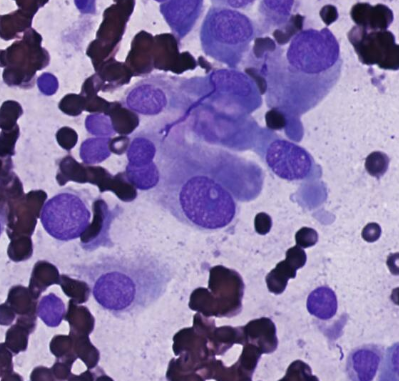
\includegraphics[scale=0.5]{image/inclusion_1.png}}
	\subfigure{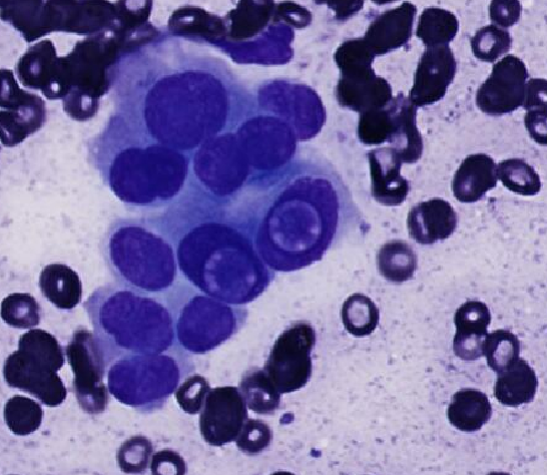
\includegraphics[scale=0.5]{image/inclusion_2.png}}
	\caption{Cells with inclusion}
	\label{fig:intro_inclu_ex}
\end{figure}

\begin{figure}
	\center
	\subfigure[Proliferative]{
		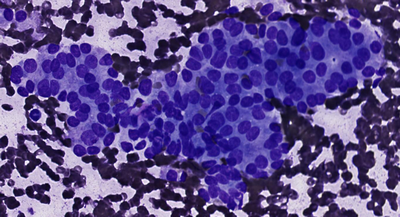
\includegraphics[scale=0.5]{image/prolif_pattern_1.png}
		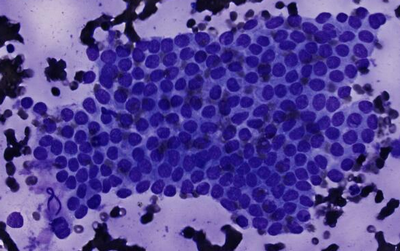
\includegraphics[scale=0.5]{image/prolif_pattern_2.png}
		\label{sfig:prolif_patterns}
	} \\
	\subfigure[Non-proliferative]{
		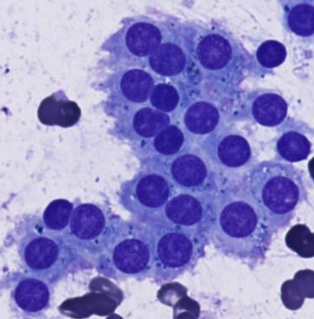
\includegraphics[scale=0.5]{image/normal_pattern_1.png}
		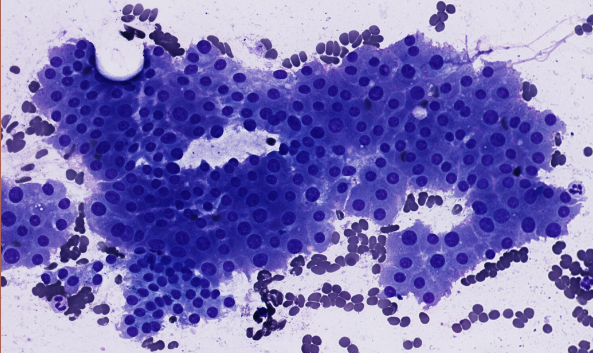
\includegraphics[scale=0.5]{image/normal_pattern_2.png}
		\label{sfig:norm_patterns}
	}
	\caption{Stained thyroid takings - architectural patterns}
	\label{fig:intro_pattern_ex}
\end{figure}


\subsubsection{Dataset}
\label{sssec:detection_thyroid_dataset}
A project dedicated to nodule malignancy detection was created on the Cytomine platform. It contains 61 annotated images with sizes ranging from 4 gigapixels to 18 gigapixels. Those images contain a total of 5921 labelled annotations performed by cytopathologists from the ULB. Those labels (or terms) link the annotations to cytological objects related to the nodule malignancy problem. The terms made available on Cytomine are organized in an ontology which is divided into three main subcategories:

\begin{itemize}
	\item \textit{Architectural patterns} : includes proliferative and non-proliferative patterns but also an intermediate class for patterns which present minor signs of proliferation.
	\item \textit{Nuclear features} : includes cells with inclusion, normal cells and some additional cell-related terms
	\item \textit{Others} : includes artefacts, background but also poly nuclear cells, red blood cells,...
\end{itemize} 

The complete ontology can be found in Appendix \ref{app:ontology}. Among those available terms, the ones that matter the most in the context of nodule malignancy detection are the cells with inclusion and the proliferative architectural patterns (major or with minor sign). The distributions of terms are given in Figure \ref{fig:ontology_histograms}.   highlights that a significant number of annotations have been made with the terms of interest but not only for these. 

\begin{figure}
	\center
	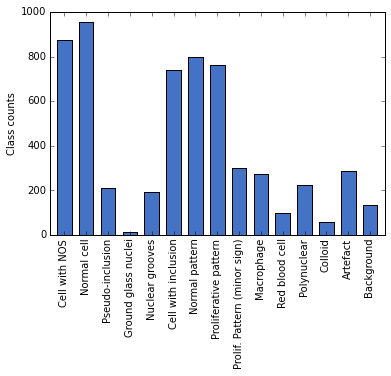
\includegraphics[scale=0.65]{image/thyroid_annotations.png}
	\caption{Annotation distribution per term in the thyroid project on Cytomine.}
	\label{fig:ontology_histograms}
\end{figure}

As far as the slide preparation is concerned, the staining technique applied is called Diff-Quick \cite{diffquick2016}. It consists in three solutions in which the glass slides must be bathed: a fixative solution, a stain and a counter-stain. This preparation typically colours cells nuclei in blue. 

\section{Computer-aided geology}
Cytology is not the only field of application where object detection algorithms can be applied. In order to assess climate variations and their effects on climate, geologists sometimes extract and analyse core samples. In  \cite{vsacre2011}, the author analyses the effects of climate variations in north Patagony based on the diatom content of core samples from Lago Bertrand and Lago Thompson. Diatoms are "\textit{algae with distinctive, transparent cell walls made of hydrated silica}" \cite{diatoms2016} (examples are given in Figure \ref{fig:diatoms}). The analysis process is the following: core samples are extracted on-site and brought back to laboratories where they are sub-sampled and smeared on microscope glass slides. The diatom concentrations are then evaluated by counting the objects. As for cytology, the process is tedious and would greatly benefit from an automated counting system. Even if counting is not the initial purpose of object detection and classification algorithms, they can be trivially extended to perform this task. Especially, as soon as the objects have been detected and classified, a program can be implemented to count the predicted classes.

\begin{figure}
	\center
	\subfigure{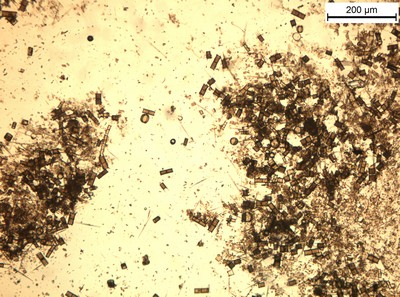
\includegraphics[scale=0.75]{image/diatomee-1.jpg}}
	\subfigure{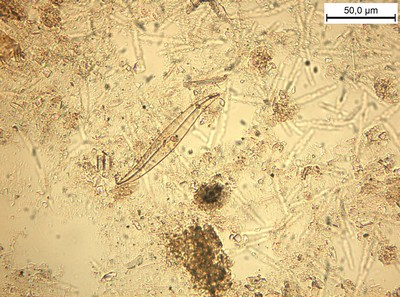
\includegraphics[scale=0.75]{image/diatomee-2.jpg}}
	\caption{Examples of diatoms (from \cite{vsacre2011}).}
	\label{fig:diatoms}
\end{figure}